\begin{frame}\frametitle{System Model}
5 d.o.f. system model is describing how the state $\vect{X}(k)$ evolves in time. It is a \textit{constant speed} model \cite{ribas10} that uses previous state $\vect{X}(k-1)$ corrupted with \textit{zero-mean} GRV with linear and angular acceleration noise  $\vect{N}(k-1)$ to make a prediction of the next state vector value (Fig. ~\ref{fig:state-tran}, Eq. ~\ref{eq:state-tran}, ~\ref{eq:f}).
\begin{equation}
\vspace{-5pt}
\vect{X}(k) = f(\vect{X}(k-1), \vect{N}(k-1))
\label{eq:f}
\end{equation}
$$\vect{N}(k) = \left[ \begin{array}{ccccc} \dot{u} & \dot{v} & \dot{w} & \ddot{\psi} & \ddot{\varphi} \end{array} \right]^{T}$$% represents the process noise consisting of linear and angular accelerations.
\vspace{-10pt}
\begin{columns}
\column{.6\textwidth}
\begin{tiny}
\begin{equation}
\begin{bmatrix} x \\ y \\ z \\ a \\ \boldsymbol{u} \\ \boldsymbol{v} \\ \boldsymbol{w} \\ \psi \\ \varphi \\ \boldsymbol{\dot{\psi}} \\ \boldsymbol{\dot{\varphi}} \end{bmatrix}_{(k)} =
\begin{bmatrix} x + (uT+\dot{u}\frac{T^{2}}{2})\cos(\psi)\cos(\varphi) - (vT+\dot{v}\frac{T^{2}}{2})\sin(\psi)\cos(\varphi) \\ 
                y + (uT+\dot{u}\frac{T^{2}}{2})\sin(\psi)\cos(\varphi) + (vT+\dot{v}\frac{T^{2}}{2})\cos(\psi)\cos(\varphi) \\ 
                z + (wT+\dot{w}\frac{T^{2}}{2})\cos(\varphi) \\ 
                a - (wT+\dot{w}\frac{T^{2}}{2})\cos(\varphi) \\ 
                \boldsymbol{u} + \dot{u}T \\ 
                \boldsymbol{v} + \dot{v}T \\ 
                \boldsymbol{w} + \dot{w}T \\ 
                \psi    + \dot{\psi}T    + \ddot{\psi}   \frac{T^{2}}{2} \\ 
                \varphi + \dot{\varphi}T + \ddot{\varphi}\frac{T^{2}}{2} \\ 
                \boldsymbol{\dot{\psi}}    + \ddot{\psi}T \\ 
                \boldsymbol{\dot{\varphi}} + \ddot{\varphi}T
\end{bmatrix}_{(k-1)} 
\label{eq:state-tran}
\end{equation} %% defined as zero-mean GRV.
\end{tiny}
\column{.35\textwidth}
\begin{figure}
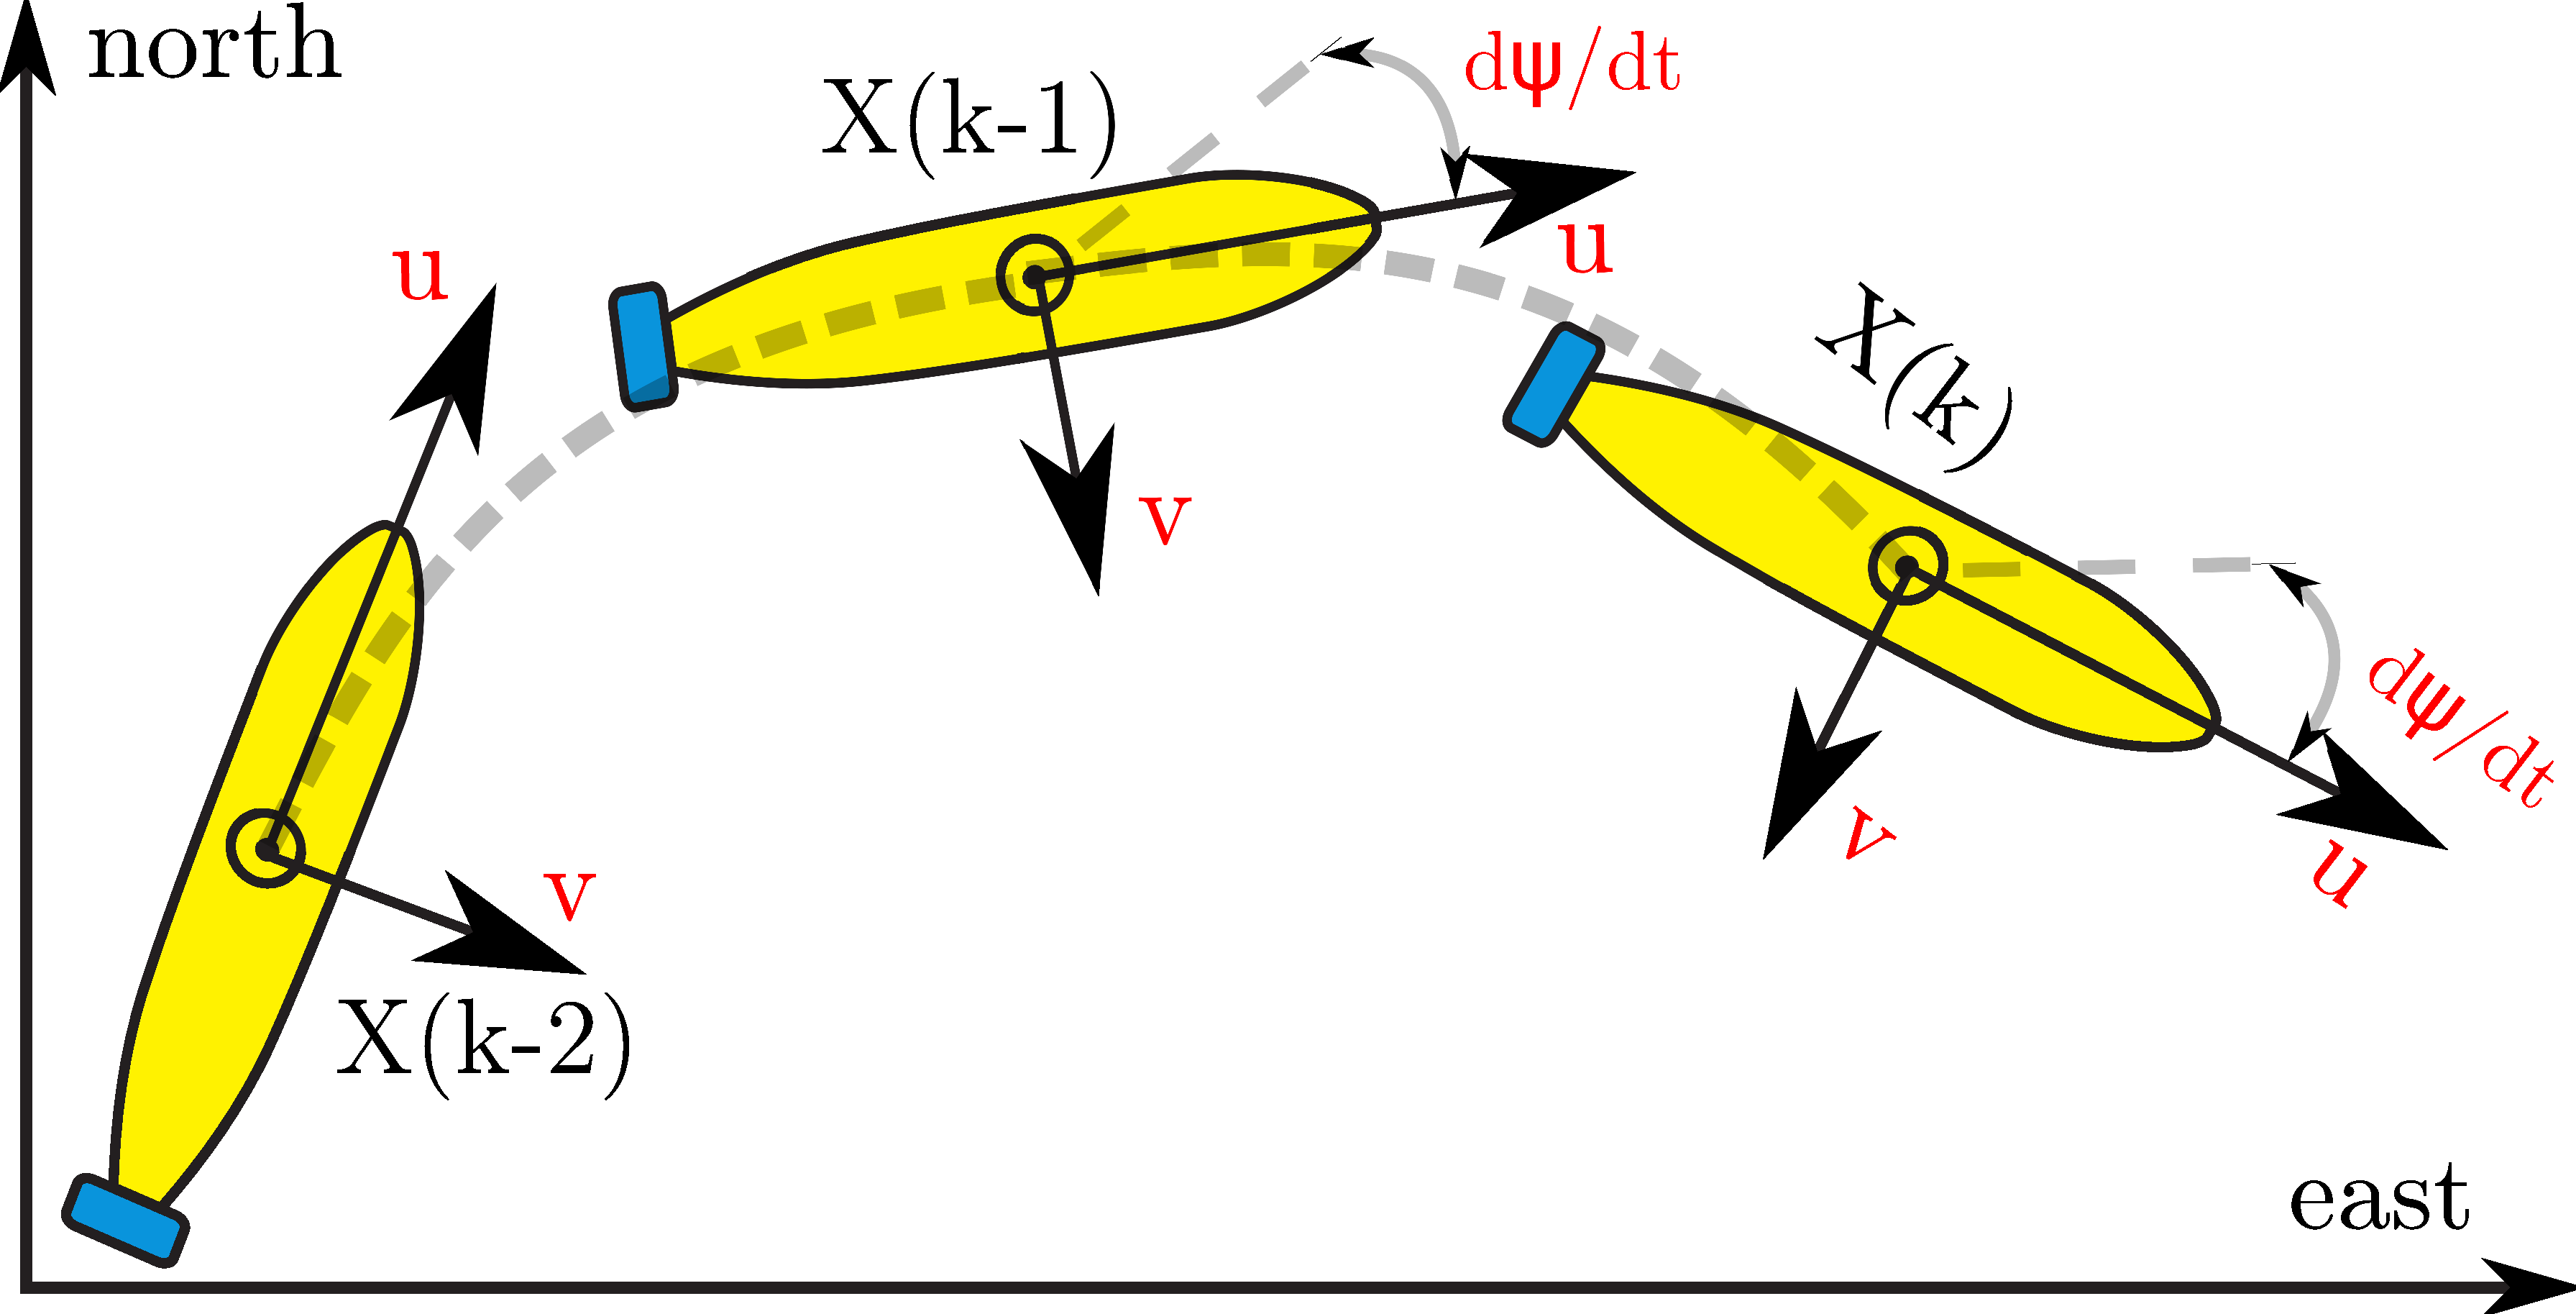
\includegraphics[width=0.98\linewidth]{fig/model.pdf}
\caption{{\scriptsize State transition model}}
\label{fig:state-tran}
\end{figure}
\end{columns}
\end{frame}